\documentclass{resume}

\tolerance=1
\emergencystretch=\maxdimen
\hyphenpenalty=10000
\hbadness=10000

\usepackage{color,hyperref}
\definecolor{darkblue}{rgb}{0.0,0.0,0.4}
\hypersetup{
    colorlinks=true,
    urlcolor=darkblue,
}
    
\begin{document}

\fontfamily{ppl}\selectfont

\noindent
\begin{tabularx}{\linewidth}{@{}m{0.8\textwidth} m{0.2\textwidth}@{}}
{
    \Large{Vasu Aggarwal} \newline
    \small{
        \clink{
            \href{mailto:vasudhruv1920@gmail.com}{vasudhruv1920@gmail.com} 
            \textbf{·} 
            {\fontdimen2\font=0.75ex +91 7859853634} 
            \textbf{·} 
            \href{https://github.com/vasu2001}{github@vasu2001}
            \textbf{·} 
            \href{https://www.linkedin.com/in/vasu-aggarwal-659b2a19a/}{linkedin@vasu-aggarwal}
            \textbf{·} 
            \href{https://www.codechef.com/users/vasu2001}{codechef@vasu2001(5 $\star$) }
            % \textbf{·} 
            % \href{https://leetcode.com/vasu2001/}{leetcode@vasu2001}
        } \newline
        Delhi, India
    }
} & 
{
    \hfill
    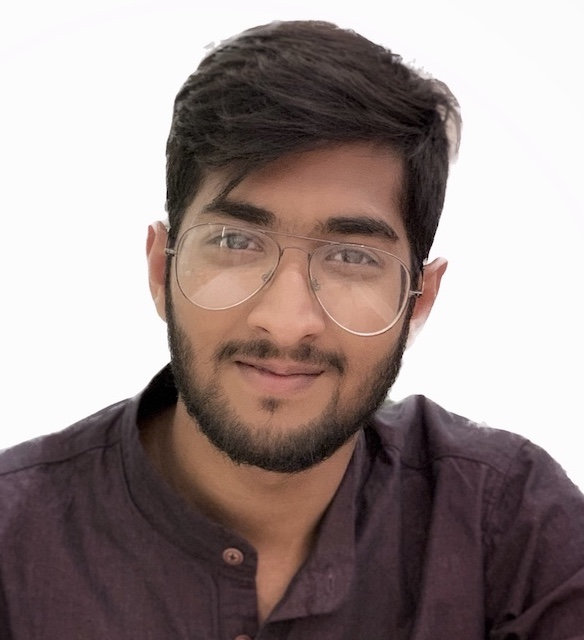
\includegraphics[width=2.8cm]{images/me.jpg}
}
\end{tabularx}

\begin{center}
\begin{tabularx}{\linewidth}{@{}m{0.7\textwidth} m{0.3\textwidth}@{}}
% left side %
{
    \csection{EXPERIENCE}{\small
        \begin{itemize}
            % item 1 %
            \item \expContent{\href{https://retailpulse.ai}{RETAIL PULSE} \hspace{5mm} \clink{\href{https://play.google.com/store/apps/details?id=club.kirana}{[Play Store]}}}
            {JAN,2022 - PRESENT}
            {REACT NATIVE INTERN}
            {
                \begin{itemize}[topsep=0pt,itemsep=0pt,parsep=0pt,partopsep=0pt]
                    \item Working on a React Native application for kirana store owners, scaled that from \textbf{1L to 3L downloads with 75K+ monthly active users}.
                    \item Technologies Used: \textbf{React Native, Redux, Firebase}
                \end{itemize}
            }

            \item \expContent{\href{https://aapkasarthi.com}{AAPKA SARTHI}\hspace{5mm} \clink{\href{https://play.google.com/store/apps/details?id=com.aapkasarthi&hl=en_IN}{[Play Store]}}}
            {AUG,2020 - DEC,2020}
            {REACT NATIVE FREELANCER}
            {
                \begin{itemize}[topsep=0pt,itemsep=0pt,parsep=0pt,partopsep=0pt]
                    \item Developed and publihed for Aapka Sarhi’s CallSpace app on Play Store, with automated continuous calling with feedback system.
                    \item Technologies Used: \textbf{React Native(TypeScript), Redux}
                \end{itemize}
            }

            % item 2 %
            \item \expContent{SOLERA LIFE SCIENCES PVT LTD}
            {MAY. 2020 - JULY, 2020}
            {REACT NATIVE INTERN}
            {
                \begin{itemize}[topsep=0pt,itemsep=0pt,parsep=0pt,partopsep=0pt]
                    \item Developed challenging end to end \textbf{chat architecture}(frontend + backend) with media sending capabilities using \textbf{WebSockets and MongoDB}.
                    % \item Built intuitive UI designs with fluid animations.
                    \item Technologies Used: \textbf{React Native, NodeJS, Redux, MongoDB, Socket.io}
                \end{itemize}
            }
        \end{itemize}
    }
    \csection{PROJECTS}{\small
        \begin{itemize}
            \item \expContent{
                CHALLENGEMII 
                \hspace{4mm} \clink{\href{https://challengemii-website.web.app/}{[Website]}}
                \hspace{2mm} \clink{\href{https://github.com/vasu2001/challengemii}{[GitHub]}} 
            }
            {APR. 2021 - JUN. 2021}
            {COMPETITION PLATFORM}
            {
                \begin{itemize}[topsep=0pt,itemsep=0pt,parsep=0pt,partopsep=0pt]
                    \item Developed and hosted a \textbf{PWA} for hosting online competitions.
                    % \item Built coin system with \textbf{admin dashboard} and referral links.
                    % \item Integrated \textbf{OAuth} login via Google, Facebook \& Twitter.
                    \item Technologies Used: \textbf{ReactJS, Firebase(Firestore, Cloud Functions, Hosting)}
                \end{itemize}
            }

            \item \expContent{
                SILENCER 
                \hspace{5mm} \clink{\href{https://www.linkedin.com/posts/vasu-aggarwal-659b2a19a_reactnative-nodejs-activity-6688436977974484992-rNLB/}{[Demo]}}
                \hspace{5mm} \clink{\href{https://github.com/vasu2001/Silencer}{[GitHub]}} 
            }
            {JUL. 2020}
            {LEARNING COMPANION}
            {
                \begin{itemize}[topsep=0pt,itemsep=0pt,parsep=0pt,partopsep=0pt]
                    \item Developed an app to learn facts effectively using Leitner System
                    % \item Built \textbf{REST api} and data models for storing all the records.
                    \item \raggedright{Technologies Used: \textbf{React Native(TypeScript), NodeJS, ExpressJS, MongoDB}}
                \end{itemize}
            }

            \item \expContent{STUED \hspace{5mm} \clink{\href{https://play.google.com/store/apps/details?id=com.stued.StuEd&hl=en_IN}{[Play Store]}}}
            {NOV. 2019 - FEB. 2020}
            {STUDY, EARN, EDUCATE}
            {
                \begin{itemize}[topsep=0pt,itemsep=0pt,parsep=0pt,partopsep=0pt]
                    \item Built an app for college students to study from their peers.
                    % \item Built backend and data architecture for storing all the records in firebase.
                    \item Integrated \textbf{in-app payments(RazorPay)} \& \textbf{Push Notifications} for reminders.
                    \item Technologies Used: \textbf{Android SDK(Java), Firebase(Auth, RealtimeDB)}
                \end{itemize}
            }
           \end{itemize}
    }


    \csection{ACHIEVEMENTS}{\small
        \begin{itemize}[topsep=5pt,itemsep=0pt,parsep=0pt,partopsep=0pt]
            \footnotesize
            \item Global Rank \textbf{37 out of 2000+} participants in CodeChef CODERS (Div. 2)
            \item Specialist at Codeforces, rating=1437, \clink{\href{https://codeforces.com/profile/vasu2001}{[vasu2001]}}
            \item Selected in \textbf{top 600 participants out of 35.5K} to attend Pulicis Sapient's JumpStart event 2021
            \item Solved \textbf{350+ questions} on Leetcode, \clink{\href{https://leetcode.com/vasu2001/}{[vasu2001]}}
            \item Authored an article on medium with \textbf{3.6K views \& 16+ hours of reading time}, \clink{\href{https://medium.com/@vasudhruv1920/react-native-catching-upto-flutter-in-performance-with-react-native-skia-a7d3395d6196}{[React Native catching upto Flutter in performance with React Native Skia]}}
            \item Organised a intercollege hackathon \clink{\href{https://www.hackinsummer.live}{[Hackin' Summer '22]}}
        \end{itemize}
    }
} 
% end left side %
& 
% right side %
{
    \csection{SKILLS}{\small
        \begin{itemize}
            \item \textbf{Technologies} \newline
            \raggedright{\footnotesize  ReactJS, React Native, Express.js, Android SDK(Java), GraphQL, SQL, MongoDB, Redux}
            % \item \textbf{Patterns \& Practices} \newline
            % \raggedright{\footnotesize Object Oriented Programming, Functional  Programming, CI \& CD, Microservices}
            \item \textbf{Languages} \newline
            \raggedright{\footnotesize JavaScript, TypeScript, C, C++, Python, Java}
            \item \textbf{Cloud Technologies} \newline
            \raggedright{\footnotesize AWS, Firebase, Vercel}
        \end{itemize}
    }
 
    \csection{EDUCATION}{\small
        \begin{itemize}
            \item \frcontent
                {BTech - CSE}
                {Jaypee Institute of Information Technology, Noida-62}
                {CGPA - 8.0 \textit{(Current)}}
                {2019 - 2023}

            \item \frcontent
                {XII - CBSE}
                {}
                {Percentage - 95.8\%}
                {2018 - 2019}
            
            \item \frcontent
                {X - CBSE}
                {}
                {CGPA - 9.8}
                {2016 - 2017}
        \end{itemize}
    }

    \csection{VOLUNTEER EXPERIENCE}{\small
       \begin{itemize}
            \item \expContent
                {Technical Coordinator}
                {SEP, 2020 – PRESENT}
                {DEVELOPER STUDENT CLUB, JIIT-62}
                {
                    \begin{itemize}[topsep=0pt,itemsep=0pt,parsep=0pt,partopsep=0pt]
                        \item Conducted a workshop on basic Web Development, taught basics of JavaScript
                        \item Developed website for \clink{\href{https://ici-conference.com}{{ICI-2022}}}
                    \end{itemize}
                }
                % {Conducted a workshop on basic Web Development, taught basics of JavaScript.}
                % {}
       \end{itemize}
    }
}

\end{tabularx}
\end{center}
\end{document}